% ============================================================
% CHAPTER 3: SYSTEM DESIGN AND ARCHITECTURE
% ============================================================
\chapter{System Design and Architecture}

This chapter presents the high-level design and architecture of the GPS spoofing detection system. We discuss design requirements, the modular system architecture, individual component roles, and the key technical innovation---the GPS--IMU consistency discriminator.

\section{Design Requirements}

The system was designed to satisfy a set of functional and non-functional requirements derived from the research objectives and practical deployment constraints of the PX4 ecosystem.

\subsection{Functional Requirements}
\begin{enumerate}
    \item \textbf{F1---Telemetry Acquisition}: Collect GPS, IMU, and vehicle state data from a PX4 flight controller at a minimum rate of 10\,Hz via the MAVLink protocol~\cite{MAVLink}.
    \item \textbf{F2---Automated Labelling}: Automatically assign binary anomaly labels to each telemetry row using physics-based heuristic rules, eliminating the need for manual annotation.
    \item \textbf{F3---Data Processing Pipeline}: Transform raw CSV telemetry logs through a five-stage pipeline: cleaning, feature engineering, labelling, windowing, and dataset splitting.
    \item \textbf{F4---Model Training}: Train and serialise Random Forest and 1D Convolutional Neural Network classifiers from the labelled dataset~\cite{Pedregosa2011, Paszke2019}.
    \item \textbf{F5---Real-Time Inference}: Perform streaming anomaly detection on live MAVLink telemetry with sub-second latency and log results for review.
    \item \textbf{F6---Management Interface}: Provide both terminal-based component lifecycle management and web-based monitoring dashboard~\cite{StreamlitDocs}.
    \item \textbf{F7---Attack Simulation}: Generate controlled GPS spoofing attacks in a PX4 SITL environment for system testing and validation.
\end{enumerate}

\subsection{Non-Functional Requirements}
\begin{itemize}
    \item \textbf{Inference latency}: Less than 100\,ms for single-window prediction.
    \item \textbf{Detection accuracy}: Target above 85\% on balanced test sets.
    \item \textbf{Sampling consistency}: Maintain stable 10\,Hz logging without dropped messages during normal and spoofed flight segments.
    \item \textbf{Software-only deployment}: No hardware augmentation or firmware modifications required.
    \item \textbf{Modularity}: Each component (monitor, pipeline, inference, UI) runs independently and can be started/stopped without affecting others.
\end{itemize}

\section{Overall System Architecture}

The system follows a modular, pipeline-oriented architecture decomposed into eight logical subsystems following the ``divide and conquer'' decomposition principle. Figure~\ref{fig:system_arch} illustrates the overall architecture and data flow.

\begin{figure}[H]
\centering
\resizebox{\textwidth}{!}{
\begin{tikzpicture}[
    node distance=1.2cm,
    block/.style={rectangle, draw, fill=blue!10, text width=3cm, text centered, minimum height=0.8cm, rounded corners, font=\small},
    data/.style={rectangle, draw, fill=gray!15, text width=2.5cm, text centered, minimum height=0.7cm, font=\footnotesize},
    arrow/.style={->, >=stealth, thick},
]
    % Simulation
    \node[block] (px4) {PX4 SITL + Gazebo};
    \node[block, right=of px4] (mavlink) {MAVLink\\UDP Bridge};
    \node[block, right=of mavlink] (monitor) {GPS Monitor\\10 Hz Logger};
    \node[data, below=of monitor] (raw) {Raw CSVs};

    % Pipeline
    \node[block, right=of monitor, xshift=1.5cm] (clean) {Data\\Cleaning};
    \node[block, right=of clean] (label) {Auto-\\Labeling};
    \node[block, right=of label] (window) {Sliding\\Windows};
    \node[block, right=of window] (train) {Model\\Training};

    % Inference
    \node[block, below=of clean, yshift=-1.5cm] (infer) {Live Inference\\Engine};
    \node[block, right=of infer] (dashboard) {Streamlit\\Dashboard};
    \node[data, below=of infer] (log) {Inference Logs};

    % Attack
    \node[block, above=of px4] (attacker) {GPS Spoofer\\Attack Injector};

    % Arrows
    \draw[arrow] (px4) -- (mavlink);
    \draw[arrow] (mavlink) -- (monitor);
    \draw[arrow] (monitor) -- (raw);
    \draw[arrow] (raw.north) -- ++(0,0.3) -| (clean);
    \draw[arrow] (clean) -- (label);
    \draw[arrow] (label) -- (window);
    \draw[arrow] (window) -- (train);
    \draw[arrow] (train.south) -- ++(0,-0.3) -| (infer);
    \draw[arrow] (infer) -- (dashboard);
    \draw[arrow] (infer) -- (log);
    \draw[arrow] (attacker) -- (px4);

\end{tikzpicture}
}
\caption{System architecture showing data flow from PX4 simulation through GPS Monitor, ML Pipeline, and Live Inference to Dashboard. The attack injector provides controlled spoofing for testing.}
\label{fig:system_arch}
\end{figure}

The data flow proceeds as follows:
\begin{enumerate}
    \item PX4 SITL generates simulated flight physics and transmits telemetry via MAVLink over UDP port 14560.
    \item The GPS Monitor connects as a MAVLink client, captures 8 message types at 10\,Hz, and writes structured CSV logs.
    \item The ML Pipeline reads raw CSV files and sequentially executes data cleaning, automated labelling, sliding window creation, and model training.
    \item Trained models (RF and CNN) are serialised to disk for use by the inference engine.
    \item The Live Inference Engine consumes streaming MAVLink telemetry, accumulates 30-sample windows, and outputs anomaly probabilities with terrain-aware model selection.
    \item The Streamlit Dashboard displays live anomaly probabilities and a GPS Trust Index gauge, with historical log replay capability.
\end{enumerate}

\section{Component Overview}

The system comprises five major runtime components and one testing utility:

\begin{description}
    \item[GPS Monitor] pymavlink-based telemetry collector. Maintains a thread-safe state model of GPS, IMU, Estimator, and Vehicle Health data. Logs structured CSV at 10\,Hz with 34 fields per record. Includes a terminal-based real-time display with telemetry preview.
    \item[ML Pipeline] Python pipeline orchestrator supporting four processing modes: \texttt{process-single} (single flight), \texttt{process-batch} (all flights in directory), \texttt{train} (model training only), and \texttt{full} (end-to-end pipeline). Configuration-driven via YAML for reproducibility.
    \item[Live Inference Engine] Streaming detector with deque-buffered 30-sample sliding windows. Loads serialised models via joblib. Applies EMA smoothing for output stability. Supports terrain-aware model dispatching. Outputs labelled CSV log with per-window anomaly probability and metadata.
    \item[Streamlit Dashboard] Web interface with two operational modes: live monitor (GPS Trust Index gauge, telemetry display, anomaly probability chart) and log replay (upload and visualise historical inference logs). Auto-refreshes from the live log file.
    \item[TUI Management Console] Textual framework application providing component lifecycle management (start/stop with PID tracking), data file browser, ML pipeline execution buttons, integrated log viewer with colour-coded output, and one-click GPS spoofing attack launch.
    \item[GPS Spoofer] MAVLink GPS\_INPUT injector connecting as companion computer (sysid=1, compid=220). Supports six attack modes: drift, ramp drift, jump+drift, static freeze, teleport, and Gaussian noise. Includes warmup phase for EKF lock-in.
\end{description}

\section{Key Innovation: GPS--IMU Consistency Check}

The core technical innovation of this system is the physics-based GPS--IMU consistency discriminator, formally defined by Equation~\ref{eq:delta_phi_full} and implemented in practice via the heuristic indicator in Equation~\ref{eq:spoof_indicator}. This section presents the formal mathematical formulation and a worked example.

\subsection{Physical Principle}

The fundamental insight underpinning the consistency check is that natural flight disturbances---wind gusts, turbulence, pilot inputs---affect both GPS and IMU sensors simultaneously. A wind gust displaces the drone physically, which changes the GPS position and is registered by the accelerometers and gyroscopes. GPS spoofing, by contrast, changes the GPS position estimate without any corresponding physical motion: the IMU registers no acceleration or rotation because the drone is not actually moving.

\begin{figure}[H]
\centering
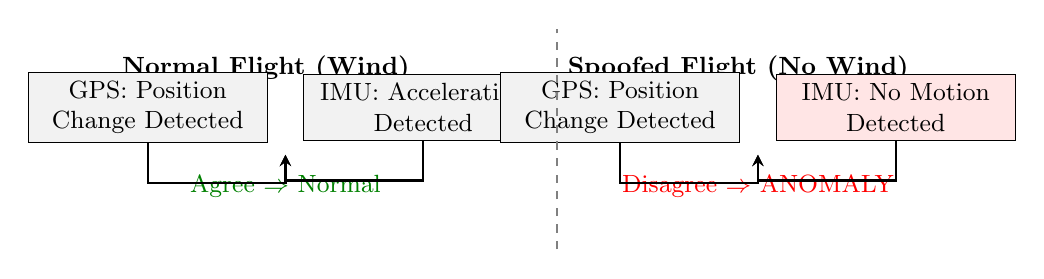
\begin{tikzpicture}[
    node distance=1.2cm,
    title/.style={font=\bfseries\small},
    sensor/.style={rectangle, draw, fill=gray!10, text width=2.8cm, text centered, minimum height=0.7cm, font=\small},
    agree/.style={font=\small\color{green!50!black}},
    disagree/.style={font=\small\color{red}},
    arrow/.style={->, >=stealth, thick},
]
    % Normal - wind
    \node[title] at (1.5, 0.5) {Normal Flight (Wind)};
    \node[sensor] (w1) at (0, 0) {GPS: Position\\Change Detected};
    \node[sensor] (w2) at (3.5, 0) {IMU: Acceleration\\Detected};
    \node[agree] at (1.75, -1) {Agree $\Rightarrow$ Normal};
    \draw[arrow] (w1.south) -- ++(0,-0.5) -| (1.75, -0.6);
    \draw[arrow] (w2.south) -- ++(0,-0.5) -| (1.75, -0.6);

    % Spoofed - no IMU
    \node[title] at (7.5, 0.5) {Spoofed Flight (No Wind)};
    \node[sensor] at (6, 0) (s1) {GPS: Position\\Change Detected};
    \node[sensor, fill=red!10] at (9.5, 0) (s2) {IMU: No Motion\\Detected};
    \node[disagree] at (7.75, -1) {Disagree $\Rightarrow$ ANOMALY};
    \draw[arrow] (s1.south) -- ++(0,-0.5) -| (7.75, -0.6);
    \draw[arrow] (s2.south) -- ++(0,-0.5) -| (7.75, -0.6);

    \draw[thick, gray, dashed] (5.2, -1.8) -- (5.2, 1);
\end{tikzpicture}
\caption{GPS--IMU consistency principle. Left: under a wind gust, both GPS and IMU detect the physical displacement---they agree. Right: under GPS spoofing, GPS reports position change while IMU registers no motion---the cross-sensor inconsistency reveals the attack.}
\label{fig:consistency_principle}
\end{figure}

This asymmetry creates a \textit{discriminative signal} that cannot be concealed by improving the spoofing waveform: regardless of how faithfully the counterfeit signal replicates authentic GPS structures, the discrepancy between GPS-reported and IMU-measured motion persists because the attacker cannot physically manipulate the drone's inertia.

\subsection{Mathematical Formulation}

Let \(\mathbf{P}_{\text{gps}, t} = (x_t, y_t, z_t)\) denote the GPS-reported position in local East-North-Up (ENU) Cartesian coordinates at time \(t\). Let \(\mathbf{a}_{\text{imu}}(t) \in \mathbb{R}^3\) denote the specific force vector measured by the IMU accelerometers, expressed in the navigation frame after gravity compensation.

The GPS--IMU consistency score over the time interval \([t_1, t_2]\) is defined as the Euclidean norm of the discrepancy between IMU-integrated displacement and GPS-reported displacement:

\begin{equation}
    \Delta \Phi(t_1, t_2) =
    \left\| \int_{t_1}^{t_2} \int_{t_1}^{\tau} \mathbf{a}_{\text{imu}}(s) \, ds \, d\tau
    \;-\; \bigl( \mathbf{P}_{\text{gps}, t_2} - \mathbf{P}_{\text{gps}, t_1} \bigr) \right\|_2
    \label{eq:delta_phi_full}
\end{equation}

The first term represents the displacement obtained by double-integrating the specific force measured by the IMU. The second term represents the displacement obtained by differencing two GPS position fixes. Under normal flight, these quantities should agree within a tolerance determined by IMU noise, gravity compensation errors, and integration drift~\cite{Hassan2023}. Under GPS spoofing, the second term reflects the attacker-controlled trajectory while the first term continues to reflect the drone's true motion.

For the heuristic implementation, this integral formulation is approximated using angular rate as a practical proxy for physical motion:

\begin{equation}
    \text{Spoofing Indicator} = \mathbb{I} \left[ \max_{i \in \{x,y,z\}} |\omega_i| < \tau_{\omega} \right]
    \;\cdot\; \mathbb{I} \left[ \| \mathbf{v}_{\text{gps}} \| > \tau_{v} \right]
    \label{eq:spoof_indicator}
\end{equation}

where \(\omega_i\) are the angular rates measured by the gyroscopes, \(\tau_{\omega} = 0.05\)\,rad/s is the quiescence threshold, and \(\tau_{v} = 5.0\)\,m/s is the GPS velocity threshold. The indicator is true only when the IMU is quiescent (no physical rotation) while GPS reports significant velocity---a condition that is physically impossible under authentic GPS but becomes true when spoofed positions are injected.

The empirical verification of this detector on the 8-flight simulation dataset, and its integration into a cascaded ML architecture, constitutes the primary experimental contribution of this research.

\subsection{Worked Numerical Example}

To make the GPS--IMU consistency principle concrete, consider two contrasting scenarios:

\textbf{Scenario A---GPS spoofing without wind.} A drone hovers at a fixed true position of $(0, 0, 20)$\,m in the local ENU frame. Over a 5-second interval, a spoofing attack injects GPS positions drifting eastward at 2\,m/s. At $t = 5$\,s, the spoofed GPS reports position $(0, 10, 20)$---a 10\,m eastward displacement. The IMU accelerometers, measuring the drone's true stationary state, register specific force near $(0, 0, 9.81)$\,m/s$^2$ (gravity only, no horizontal acceleration). Double-integrating yields IMU-estimated displacement $(0, 0, 0)$\,m. The GPS--IMU consistency score (Equation~\ref{eq:delta_phi_full}) evaluates to:

\[
\Delta \Phi = \| (0, 0, 0) - (0, 10, 0) \|_2 = 10\text{ m}
\]

which substantially exceeds the typical noise floor of the consistency score under normal flight (approximately 1--2\,m from IMU integration drift), correctly identifying the spoofing.

\textbf{Scenario B---Wind gust without spoofing.} The same drone experiences a 5\,m/s wind gust from the north at $t = 0$. The wind displaces the drone southward by 2\,m over 5 seconds: GPS reports $(0, -2, 20)$. The IMU registers the aerodynamic forces: horizontal acceleration of approximately 0.5\,m/s$^2$ from the induced body tilt (the quadcopter pitches to counteract drift). Double-integrating this acceleration yields IMU-estimated displacement approximately $(0, -1.8, 0)$\,m (the 0.2\,m discrepancy arises from IMU noise). The consistency score evaluates to:

\[
\Delta \Phi = \| (0, -1.8, 0) - (0, -2, 0) \|_2 = 0.2\text{ m}
\]

which is well within the typical 1--2\,m noise floor expected from IMU integration drift over a 5-second interval, correctly identifying the GPS data as authentic despite the environmental disturbance. This contrast illustrates the discriminative power of the consistency check: it distinguishes the asymmetric effect of spoofing (GPS moves, IMU does not) from the symmetric effect of wind (both sensors register the physical displacement).
